\documentclass[letterpaper, 24pt, final, onecolumn, titlepage] {article}


\usepackage{enumerate}
\usepackage{graphicx}
\usepackage{listings}
\usepackage{color}
\usepackage{setspace}
\usepackage {amsmath}
\usepackage{amssymb}
\usepackage{verbatim}
\usepackage{afterpage}
\usepackage{geometry}
\usepackage{hyperref}

\hypersetup{
  colorlinks, linkcolor=red
}
\geometry{
 a4paper,
 total={170mm,257mm},
 left=1cm,
 right=1cm,
 }
\title{ECE 270: Computer Methods in ECE \\
	\vspace{1.5cm}
   		\begin{center}\includegraphics{umlogo} \end{center}
	\vspace{1.5cm}
	\textbf{Quiz \#11} \\
	Rectangle Eating Game}
	
\author{Hussein El-Souri}

\date{\today}

\definecolor{dkgreen}{rgb}{0,0.6,0}
\definecolor{gray}{rgb}{0.5,0.5,0.5}
\definecolor{mauve}{rgb}{0.58,0,0.82}


\lstset{frame=tb,
  language=C,
  aboveskip=3mm,
  belowskip=3mm,
  showstringspaces=false,
  columns=flexible,
  basicstyle={\small\ttfamily},
  numbers=none,
  numberstyle=\tiny\color{gray},
  keywordstyle=\color{blue},
  commentstyle=\color{dkgreen},
  stringstyle=\color{mauve},
  breaklines=true,
  breakatwhitespace=true,
  tabsize=3
}

\begin{document}

\maketitle

\doublespacing

\section{Statement of the Problem}

We wish to create a rectangle that increases in size whenever it intersects with other rectangles.
\section{Description of Solution}

First we have to create a rectangle using the ofRectangle and also an array of rectangles using the same class.\\
Next we set up a boolean variable to check for intersections and also integers for colors, length,width, position, count and finally an array of integers that determin if the array of rectangles are visible.
we setup a loop to first initiallizethe array of rectangles to random locations and sizes. We also setup an array to determin if there are any intersections betwen our rectangle and the visible rectangles when an intersection happens the visible rectangles are made invisible.
The draw function is set up according to a loop to draw the visible rectangles.


\section{Testing and Output}
\begin{center}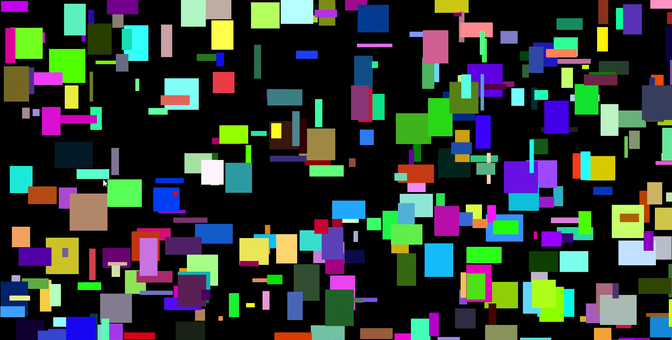
\includegraphics{capture1} \end{center}
\begin{center}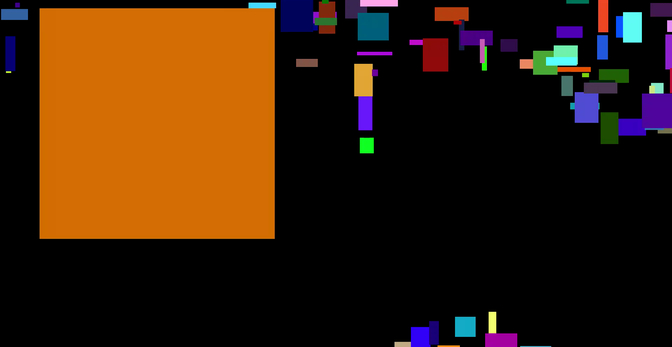
\includegraphics{capture2} \end{center}


\section{Code}
\singlespacing

\begin{lstlisting}

//----ofApp.h content
ofRectangle player;
ofRectangle food[250];
unsigned int red,green,blue;
bool check;
ofSoundPlayer myMusic;
int isVisible[250];
int i;
int length=20,width=40,number=0,randLength=0,randWidth=0,randX=0,randY=0;
//--------------------------------

//--ofApp.cpp content
void ofApp::setup(){
ofBackground(0);
ofSetFrameRate(20);
for(i=0;i<250;i++)
{
    randLength = 10+ rand()% 100;
    randWidth = 10 + rand()% 100;
    randX = rand()% 1921;
    randY= rand()% 1081;
    isVisible[i]=1;
    food[i].set(randX,randY,randWidth,randLength);
    player.setHeight(length);
    player.setWidth(width);
}
myMusic.loadSound("Casin.mp3",0);
myMusic.play();
}
//--------------------------------------------------------------






void ofApp::update(){
for (i=0;i<250;i++)
{
    if(isVisible[i]==1)
    {
        check=player.intersects(food[i]);
        if(check==1)
        {
            number=number+1;
            player.setWidth(width+number);
            player.setHeight(length+number);
            isVisible[i]=0;
        }
    }
}
}

//--------------------------------------------------------------
void ofApp::draw(){
ofRect(player);
for(i=0;i<250;i++)
{

    if(isVisible[i]==1)
    {
        red= rand()%256;
        green= rand()%256;
        blue= rand()%256;
        ofSetColor(red,green,blue);
        ofRect(food[i]);
    }
}
}
void ofApp::mouseMoved(int x, int y){
player.setX(x);
player.setY(y);
}
\end{lstlisting}

\end{document}